% Options for packages loaded elsewhere
\PassOptionsToPackage{unicode}{hyperref}
\PassOptionsToPackage{hyphens}{url}
%
\documentclass[
  ignorenonframetext,
]{beamer}
\usepackage{pgfpages}
\setbeamertemplate{caption}[numbered]
\setbeamertemplate{caption label separator}{: }
\setbeamercolor{caption name}{fg=normal text.fg}
\beamertemplatenavigationsymbolsempty
% Prevent slide breaks in the middle of a paragraph
\widowpenalties 1 10000
\raggedbottom
\setbeamertemplate{part page}{
  \centering
  \begin{beamercolorbox}[sep=16pt,center]{part title}
    \usebeamerfont{part title}\insertpart\par
  \end{beamercolorbox}
}
\setbeamertemplate{section page}{
  \centering
  \begin{beamercolorbox}[sep=12pt,center]{part title}
    \usebeamerfont{section title}\insertsection\par
  \end{beamercolorbox}
}
\setbeamertemplate{subsection page}{
  \centering
  \begin{beamercolorbox}[sep=8pt,center]{part title}
    \usebeamerfont{subsection title}\insertsubsection\par
  \end{beamercolorbox}
}
\AtBeginPart{
  \frame{\partpage}
}
\AtBeginSection{
  \ifbibliography
  \else
    \frame{\sectionpage}
  \fi
}
\AtBeginSubsection{
  \frame{\subsectionpage}
}
\usepackage{amsmath,amssymb}
\usepackage{lmodern}
\usepackage{iftex}
\ifPDFTeX
  \usepackage[T1]{fontenc}
  \usepackage[utf8]{inputenc}
  \usepackage{textcomp} % provide euro and other symbols
\else % if luatex or xetex
  \usepackage{unicode-math}
  \defaultfontfeatures{Scale=MatchLowercase}
  \defaultfontfeatures[\rmfamily]{Ligatures=TeX,Scale=1}
\fi
\usetheme[]{Berkeley}
\usecolortheme{whale}
\usefonttheme{structurebold}
% Use upquote if available, for straight quotes in verbatim environments
\IfFileExists{upquote.sty}{\usepackage{upquote}}{}
\IfFileExists{microtype.sty}{% use microtype if available
  \usepackage[]{microtype}
  \UseMicrotypeSet[protrusion]{basicmath} % disable protrusion for tt fonts
}{}
\makeatletter
\@ifundefined{KOMAClassName}{% if non-KOMA class
  \IfFileExists{parskip.sty}{%
    \usepackage{parskip}
  }{% else
    \setlength{\parindent}{0pt}
    \setlength{\parskip}{6pt plus 2pt minus 1pt}}
}{% if KOMA class
  \KOMAoptions{parskip=half}}
\makeatother
\usepackage{xcolor}
\newif\ifbibliography
\usepackage{longtable,booktabs,array}
\usepackage{calc} % for calculating minipage widths
\usepackage{caption}
% Make caption package work with longtable
\makeatletter
\def\fnum@table{\tablename~\thetable}
\makeatother
\usepackage{graphicx}
\makeatletter
\def\maxwidth{\ifdim\Gin@nat@width>\linewidth\linewidth\else\Gin@nat@width\fi}
\def\maxheight{\ifdim\Gin@nat@height>\textheight\textheight\else\Gin@nat@height\fi}
\makeatother
% Scale images if necessary, so that they will not overflow the page
% margins by default, and it is still possible to overwrite the defaults
% using explicit options in \includegraphics[width, height, ...]{}
\setkeys{Gin}{width=\maxwidth,height=\maxheight,keepaspectratio}
% Set default figure placement to htbp
\makeatletter
\def\fps@figure{htbp}
\makeatother
\setlength{\emergencystretch}{3em} % prevent overfull lines
\providecommand{\tightlist}{%
  \setlength{\itemsep}{0pt}\setlength{\parskip}{0pt}}
\setcounter{secnumdepth}{-\maxdimen} % remove section numbering
\AtBeginSubsection{}
\AtBeginSection{}
\definecolor{unbc}{HTML}{035642}
\setbeamercolor{structure}{fg=unbc}
\setbeamertemplate{navigation symbols}{}
\setbeamertemplate{footline}[page number]
\ifLuaTeX
  \usepackage{selnolig}  % disable illegal ligatures
\fi
\IfFileExists{bookmark.sty}{\usepackage{bookmark}}{\usepackage{hyperref}}
\IfFileExists{xurl.sty}{\usepackage{xurl}}{} % add URL line breaks if available
\urlstyle{same} % disable monospaced font for URLs
\hypersetup{
  pdftitle={Research Proposal},
  pdfauthor={Akihiko Mori, MA NRES UNBC},
  hidelinks,
  pdfcreator={LaTeX via pandoc}}

\title{Research Proposal}
\subtitle{Measuring Food Waste in Prince George Restaurant: Volume,
Model, and Effects}
\author{Akihiko Mori, MA NRES UNBC}
\date{January 01, 2023}

\begin{document}
\frame{\titlepage}

\begin{frame}[allowframebreaks]
  \tableofcontents[hideallsubsections]
\end{frame}
\hypertarget{introduction}{%
\section{Introduction}\label{introduction}}

\begin{frame}{Introduction}
\protect\hypertarget{introduction-1}{}
Food Loss and Waste (FLW) happens everywhere.

\begin{itemize}
\tightlist
\item
  One-third of food is lost or wasted around the world{[}1{]}.
\item
  Around 1.3 billion tons of FWL is generated annually, and the rate is
  projected to grow by 44\% per year by 2025{[}2{]}.
\end{itemize}

\begin{itemize}
\tightlist
\item
  Canada creates about 35 million tons and the largest waste generator
  per capita in western countries in 2016{[}3{]}.
\item
  Canada's avoidable FLW is 49.5 million CAD{[}4{]}.
\end{itemize}
\end{frame}

\begin{frame}{Introduction}
\protect\hypertarget{introduction-2}{}
\begin{itemize}
\tightlist
\item
  In BC, 40\% of the waste to landfills is organic waste, the majority
  is produced from domestic waste{[}5{]}.
\end{itemize}

\begin{itemize}
\tightlist
\item
  Recent huge discoveries in the food waste research focus on waste
  generated by households:{[}6,7,8,9{]}.
\end{itemize}

\begin{itemize}
\tightlist
\item
  Limited number of studies done on the food supply side.
\item
  Even little esimations of FLW in food service industry.
\end{itemize}
\end{frame}

\begin{frame}{Introduction}
\protect\hypertarget{introduction-3}{}
\begin{block}{Research Questions}
\protect\hypertarget{research-questions}{}
\begin{itemize}
\tightlist
\item
  What is the average volume of food that is wasted during processing
  and consumption in restaurants?
\item
  What is the extent of food wastage in Japanese restaurants in Prince
  George?
\item
  What are the main factors contributing to food loss and waste?
\item
  To what extent is a social or environmental impact from food loss
  waste generated by a single restaurant?
\item
  What approaches are Japanese restaurant operators taking to reduce
  food waste generation?
\end{itemize}
\end{block}
\end{frame}

\hypertarget{literature-review}{%
\section{Literature Review}\label{literature-review}}

\begin{frame}{Literature Review}
\protect\hypertarget{literature-review-1}{}
\begin{block}{Definition of FLW}
\protect\hypertarget{definition-of-flw}{}
\begin{itemize}
\tightlist
\item
  No universally accepted definitions of FLW
\end{itemize}

\begin{longtable}[]{@{}ll@{}}
\toprule()
Organizations & Definition \\
\midrule()
\endhead
Food Loss by FAO & harvest/slaughter/catch \\
Food Waste by FAO & retail/ consumption \\
Food Waste by EU & Food removed from FSC \\
Food Loss by US & unused product from agri \\
Food Waste by US & Subcomponent of FL \\
\bottomrule()
\end{longtable}

(Source {[}10{]})
\end{block}
\end{frame}

\begin{frame}{Literature Review}
\protect\hypertarget{literature-review-2}{}
\begin{block}{Definition of FLW}
\protect\hypertarget{definition-of-flw-1}{}
\begin{longtable}[]{@{}lllll@{}}
\toprule()
1 & 2 & 3 & 4 & 5 \\
\midrule()
\endhead
Production & Handling & Process & Distribution & Consumption \\
\textless--- & --- & FLW & --- & ---\textgreater{} \\
\textless--- & FL & ---\textgreater{} & \textless--- & FW
---\textgreater{} \\
\bottomrule()
\end{longtable}

\begin{longtable}[]{@{}llll@{}}
\toprule()
Organizations & FL & FW & Subset \\
\midrule()
\endhead
FAO & First 3 stages & Last 2 stages & X \\
EU & None & All & X \\
US & All & Last 2 stages & O \\
\bottomrule()
\end{longtable}
\end{block}
\end{frame}

\begin{frame}{Literature Review}
\protect\hypertarget{literature-review-3}{}
\begin{block}{Definition of FLW}
\protect\hypertarget{definition-of-flw-2}{}
\begin{longtable}[]{@{}lll@{}}
\toprule()
& Edible & Inedible \\
\midrule()
\endhead
Solid & FL & FW \\
Liquid & FW & X \\
\bottomrule()
\end{longtable}
\end{block}
\end{frame}

\begin{frame}{Literature Review}
\protect\hypertarget{literature-review-4}{}
\begin{block}{Definition of FLW}
\protect\hypertarget{definition-of-flw-3}{}
\begin{itemize}
\tightlist
\item
  Food Loss: generated by provider
\item
  Food Waste: generated by consumers
\end{itemize}

\begin{figure}
\centering
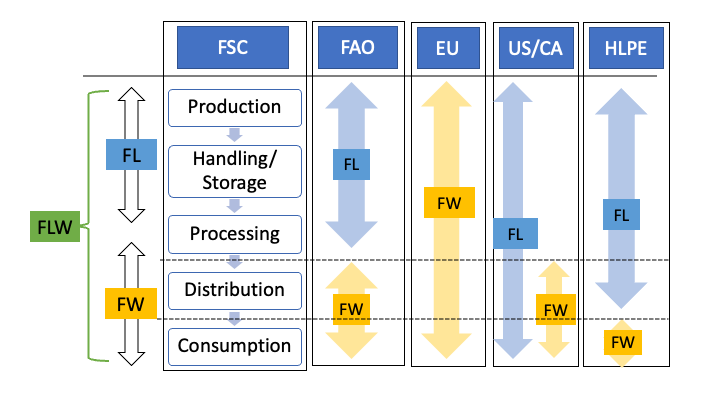
\includegraphics[width=0.9\textwidth,height=\textheight]{defnFLW.png}
\caption{Flow of FLW}
\end{figure}
\end{block}
\end{frame}

\begin{frame}{Literature Review}
\protect\hypertarget{literature-review-5}{}
\begin{block}{Five Measurements of FLW}
\protect\hypertarget{five-measurements-of-flw}{}
\begin{longtable}[]{@{}ll@{}}
\toprule()
Method & Note \\
\midrule()
\endhead
1.Self-report & individuals report FLW \\
& low cost but high dropouts \\
2.Survey & collect FLW by interview or questionnaire \\
& cost-effective but not accurate \\
3.Composition & sample and analysis at lab \\
& need special knowledge and equipment \\
4.Mass balance & material flow analysis \\
& limitation in waste factor assumptions \\
5.\textbf{Direct weight} & directly measure FLW \\
& most accurate but high cost \\
\bottomrule()
\end{longtable}
\end{block}
\end{frame}

\begin{frame}{Literature Review}
\protect\hypertarget{literature-review-6}{}
\begin{block}{Statistic Model}
\protect\hypertarget{statistic-model}{}
\begin{itemize}
\item
  \textbf{Multiple Linear Regression}
\item
  Ad: Simple and interpretable
\item
  Disad: Not suitable to time series
\item
  Disad: Stationary and Spurious
\item
  \textbf{Bayesian Modelling}
\item
  Ad: Flexible and adaptable to time series data
\item
  Disad: No appropriate result in some cases
\end{itemize}
\end{block}
\end{frame}

\begin{frame}{Literature Review}
\protect\hypertarget{literature-review-7}{}
\begin{block}{Effects of Food Loss and Waste}
\protect\hypertarget{effects-of-food-loss-and-waste}{}
\begin{itemize}
\item
  \textbf{Economic Loss}:
\item
  labour, material resources, time, and energy
\item
  \textbf{Environmental Impacts}:
\item
  water pollution, deforestation, soil erosion, and GHG
\end{itemize}

Reducing FLW can mitigate these economic and environmental impacts.
Through better supply chain management, reducing consumer food waste,
and increasing food recovery.
\end{block}
\end{frame}

\begin{frame}{Literature Review}
\protect\hypertarget{literature-review-8}{}
\begin{block}{Hypotheses}
\protect\hypertarget{hypotheses}{}
\begin{itemize}
\tightlist
\item
  Estimate average FLW
\item
  Any patterns between FLW and business operations
\item
  Any patterns between FLW and weather conditions
\item
  Estimate economic and environmental impacts
\end{itemize}
\end{block}
\end{frame}

\hypertarget{methods}{%
\section{Methods}\label{methods}}

\begin{frame}{Methods}
\protect\hypertarget{methods-1}{}
\begin{block}{Study Area}
\protect\hypertarget{study-area}{}
\begin{itemize}
\tightlist
\item
  Japanese restaurant located a suburban area of Prince George
\item
  lunch and dinner for three hours each
\item
  six days of a week: from Tuesday to Sunday
\end{itemize}

\begin{figure}
\centering
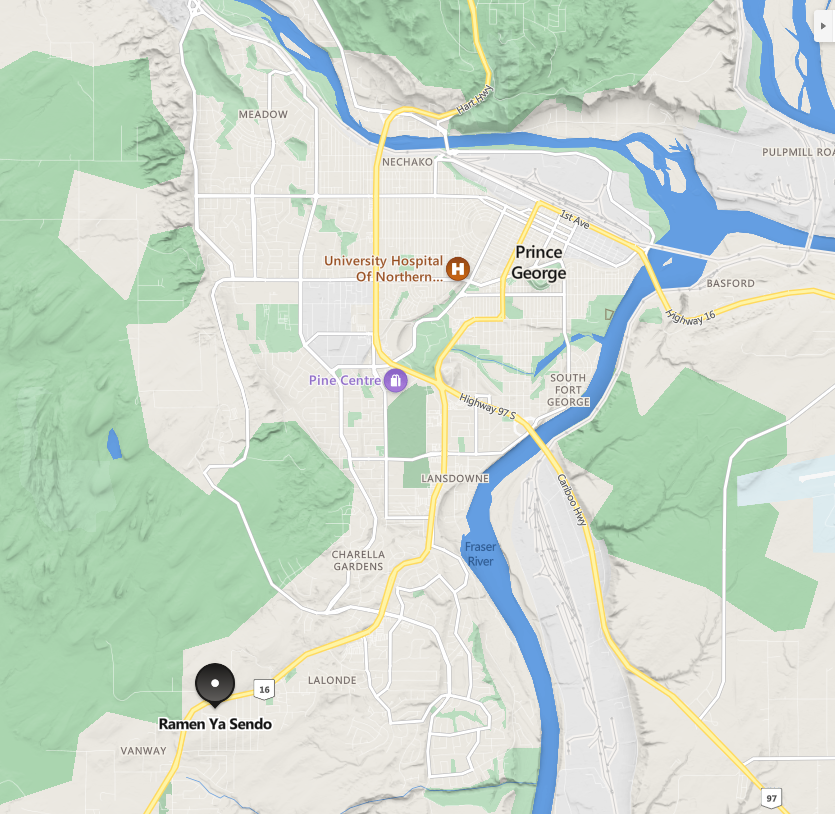
\includegraphics[width=0.35\textwidth,height=\textheight]{sendoMap.png}
\caption{Research Location Site}
\end{figure}
\end{block}
\end{frame}

\begin{frame}{Methods}
\protect\hypertarget{methods-2}{}
\begin{block}{Sample Collection}
\protect\hypertarget{sample-collection}{}
\begin{longtable}[]{@{}cc@{}}
\toprule()
Busket for Food Loss & Busket and Strainer for Food Waste \\
\midrule()
\endhead
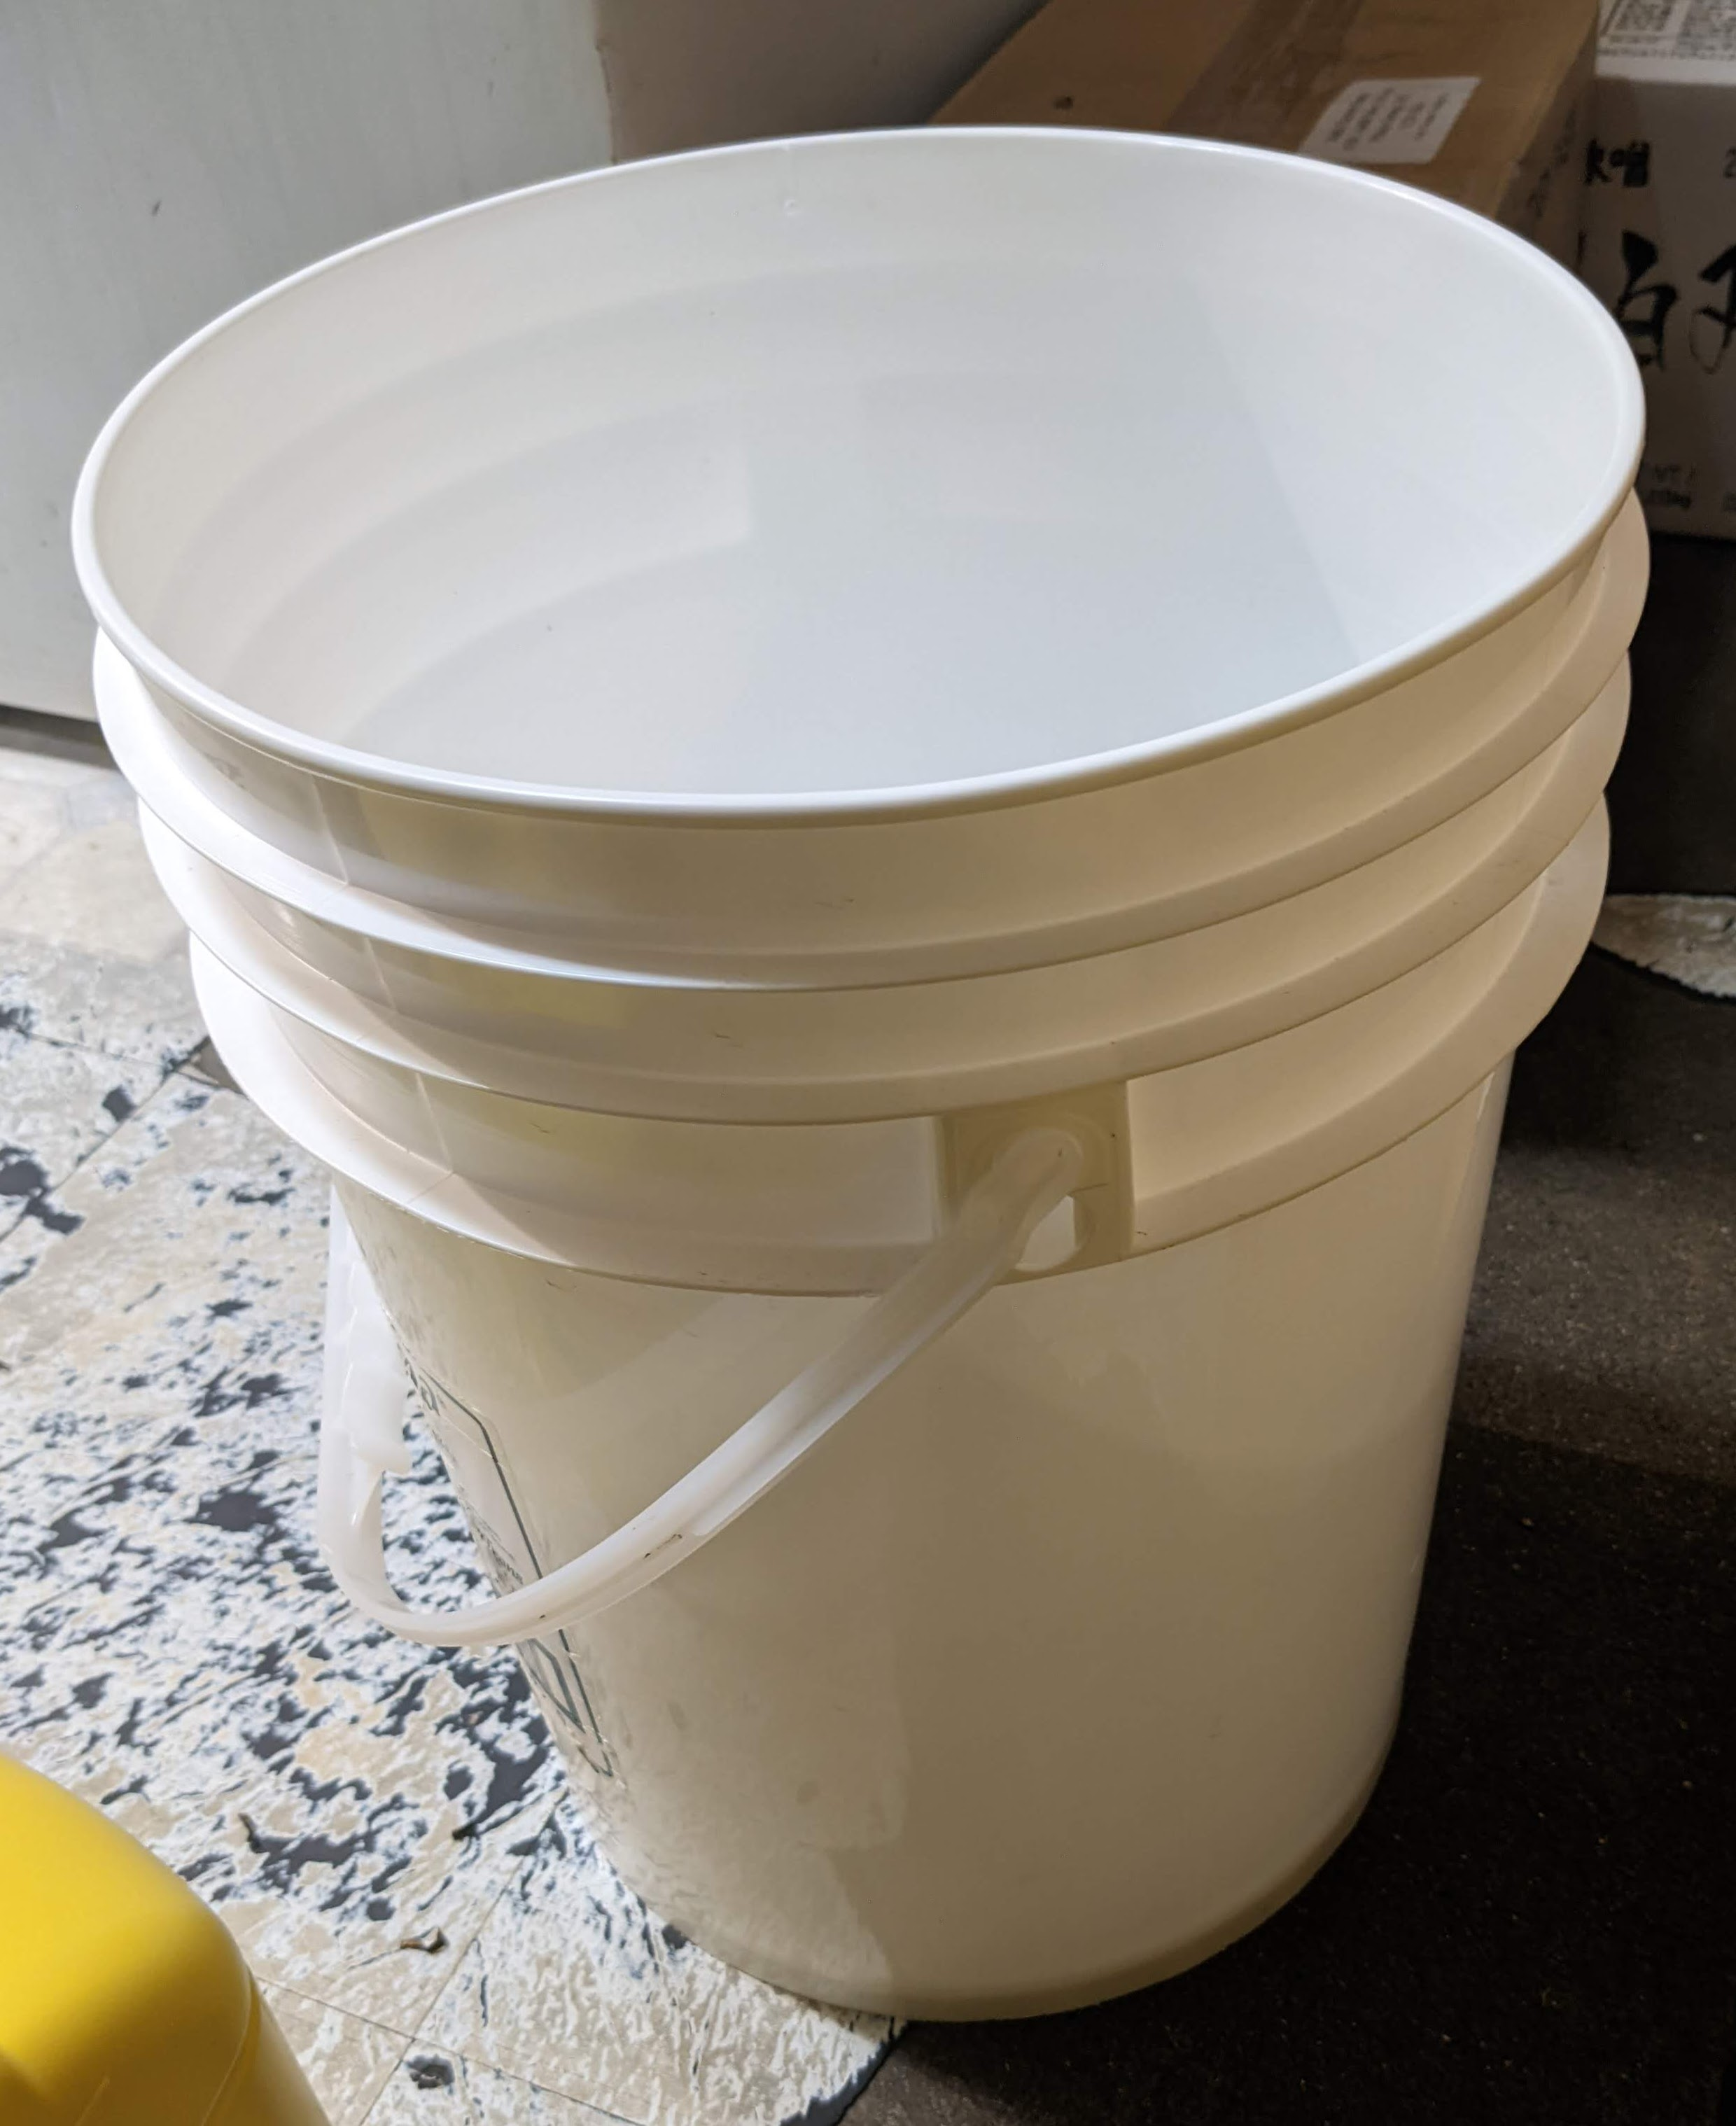
\includegraphics[width=0.3\textwidth,height=\textheight]{busket.jpg} &
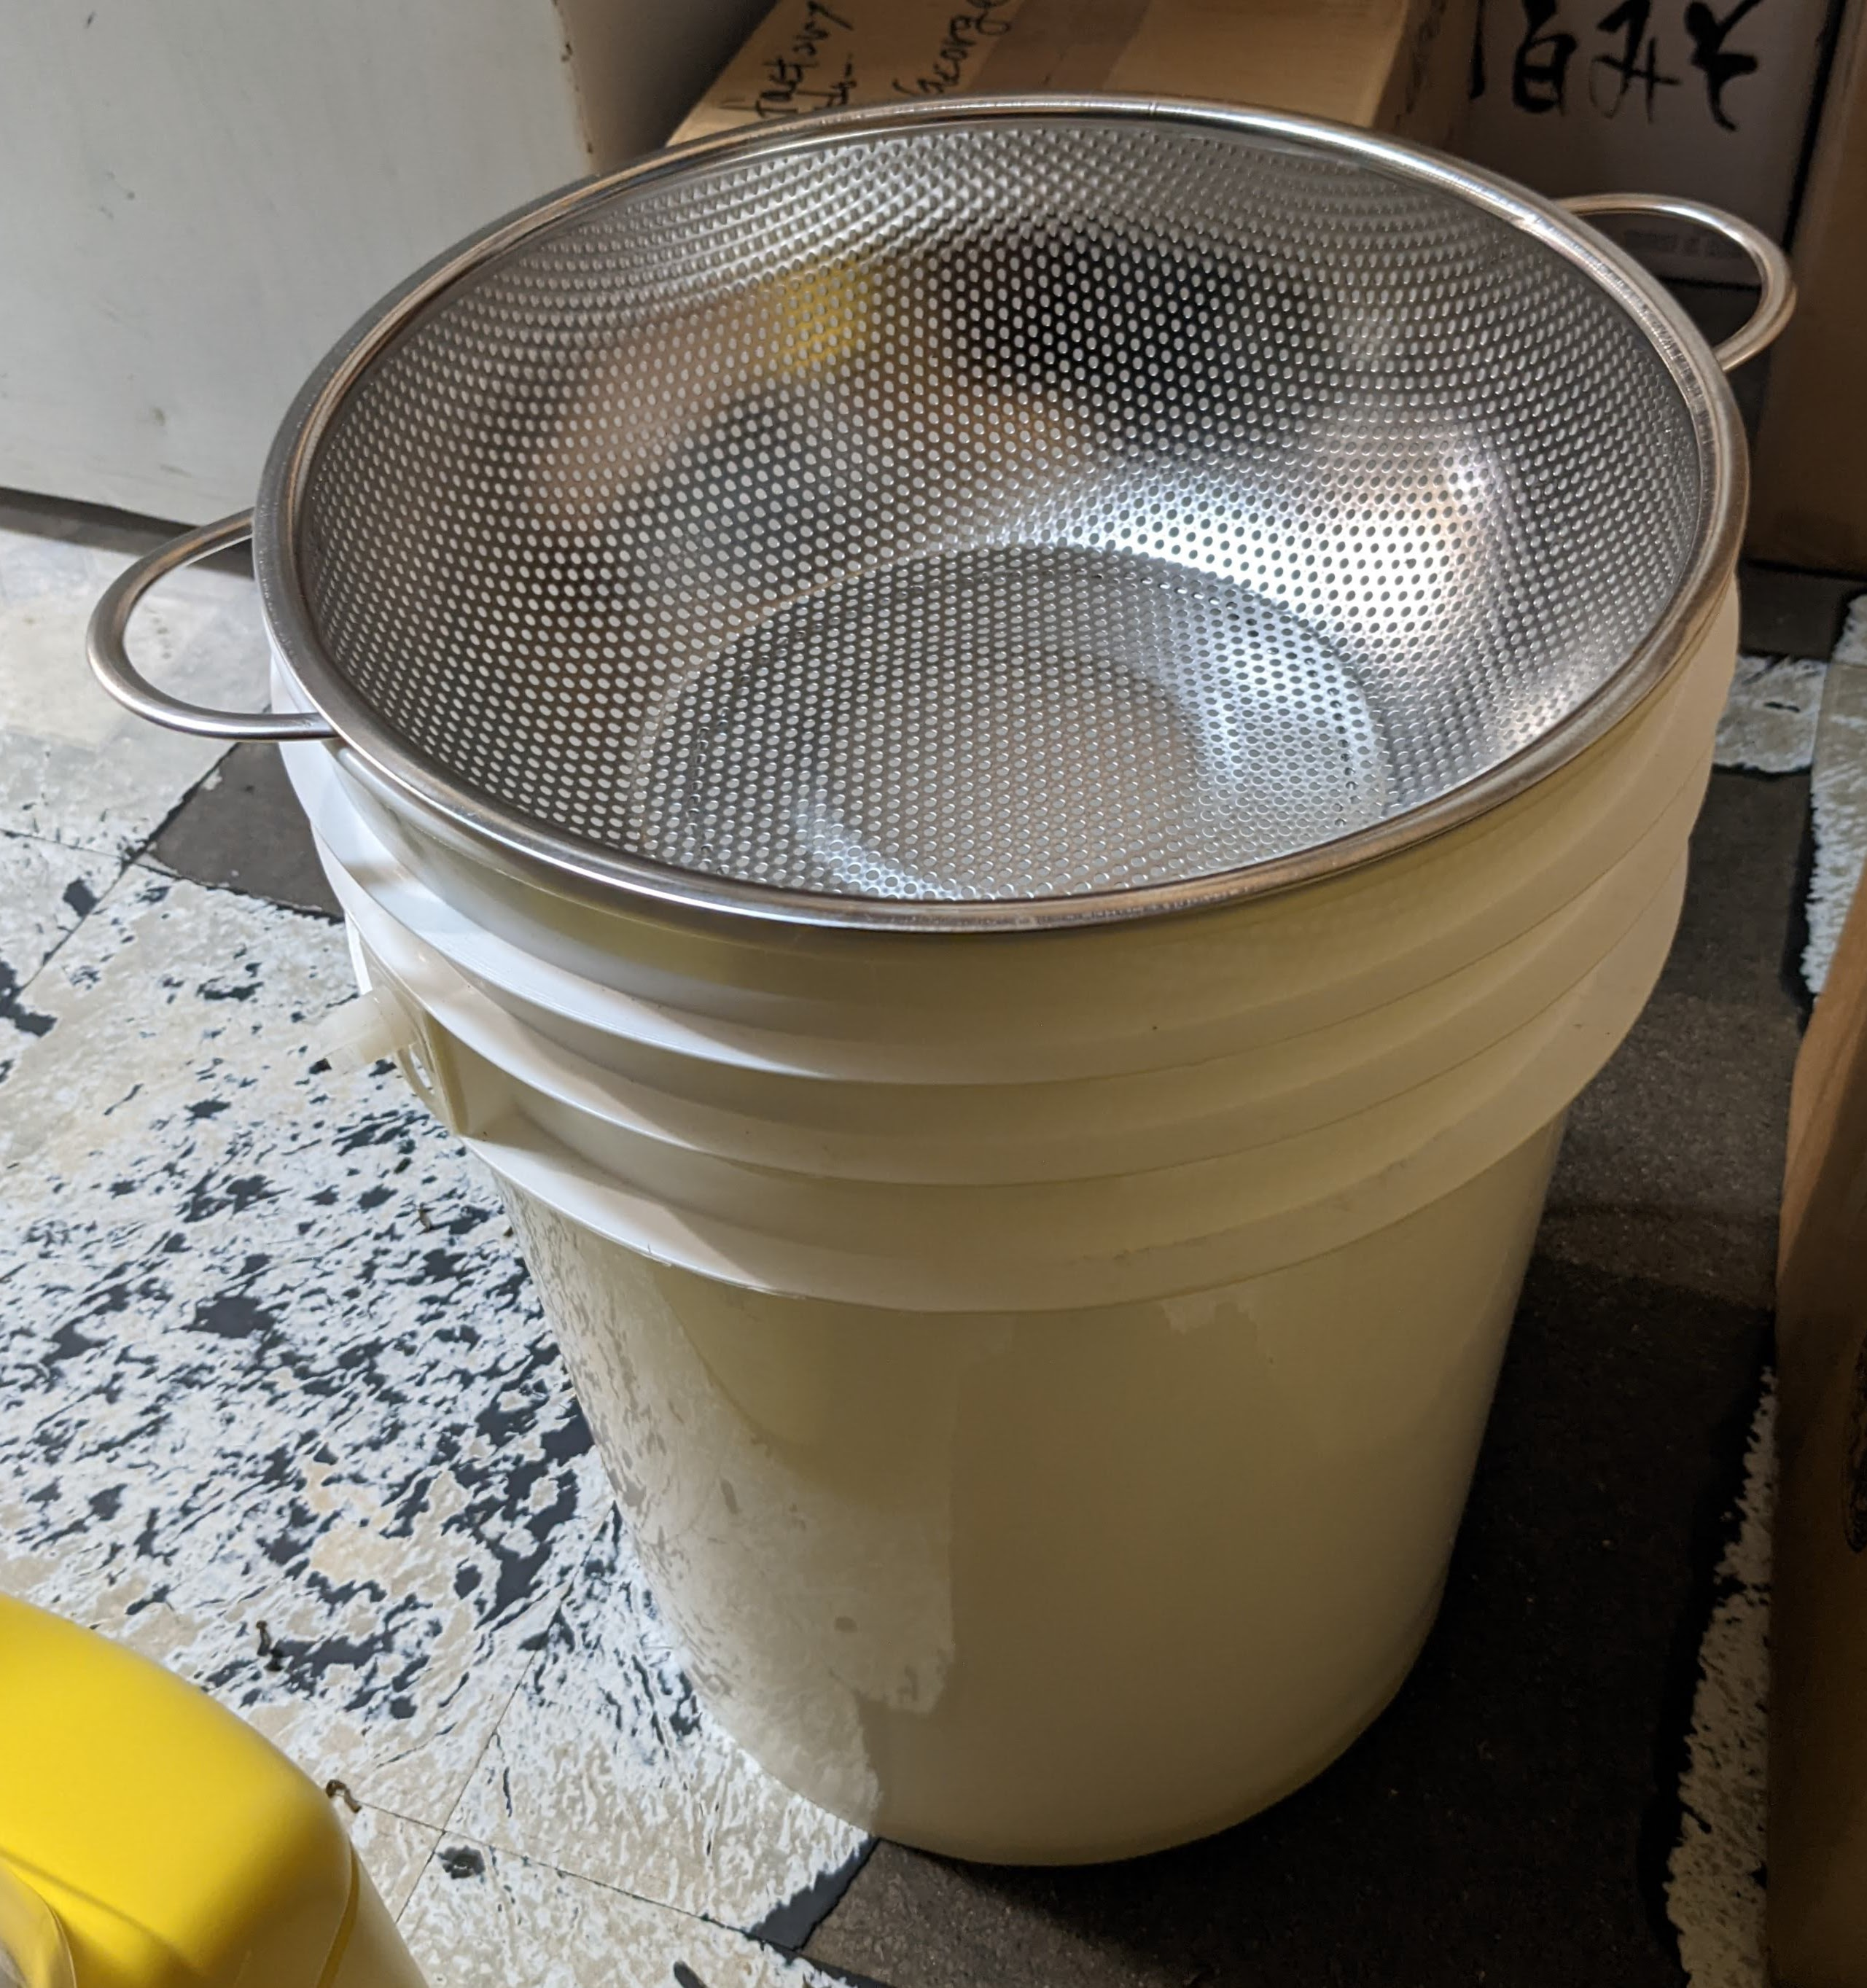
\includegraphics[width=0.35\textwidth,height=\textheight]{busketStrainer.jpg} \\
\bottomrule()
\end{longtable}
\end{block}
\end{frame}

\begin{frame}{Methods}
\protect\hypertarget{methods-3}{}
\begin{block}{Sample Size}
\protect\hypertarget{sample-size}{}
\begin{itemize}
\tightlist
\item
  \textbf{Power analysis}, 95\% CI and 20\% margin of error with 10
  explanatory variables says 110 samples.
\item
  \textbf{Rule-of-thumb}, one in ten rule suggests 100 observations with
  10 predictors{[}11{]}
\item
  Green's rule states 130 samples with 10 predictors{[}12{]}
\end{itemize}
\end{block}
\end{frame}

\begin{frame}{Methods}
\protect\hypertarget{methods-4}{}
\begin{block}{Variables}
\protect\hypertarget{variables}{}
\begin{longtable}[]{@{}ll@{}}
\toprule()
Variables & Note \\
\midrule()
\endhead
1.Food Loss & Daily disposed food by kitchen \\
2.Liquid Food Waste & Daily disposed liquid food by customers \\
3.Solid Food Waste & Daily disposed solid food by customers \\
4.Number of Customers & Daily Number of dine-in customers \\
5.Sales & Daily sales \\
6.Liquor & Daily Number of liquors sold \\
7.Takeouts & Daily Number of takeout sold \\
8.Orders & Daily Number of orders sold \\
9.Temperature & Hourly mean temperature each day \\
10.Humidity & Hourly mean humidity each day \\
11.Precipitation & Precipitation each day \\
\bottomrule()
\end{longtable}
\end{block}
\end{frame}

\begin{frame}{Methods}
\protect\hypertarget{methods-5}{}
\begin{block}{Multiple Linear Regression Model (additive)}
\protect\hypertarget{multiple-linear-regression-model-additive}{}
\[
\begin{aligned}
Y &=  X\beta + \epsilon\\
\epsilon_i &\overset{\text{i.i.d.}}{\sim} N(\mu=0, \sigma^2).
\end{aligned}
\]
\end{block}

\begin{block}{Baysian Modelling}
\protect\hypertarget{baysian-modelling}{}
\[
\begin{aligned}
Y &= X\beta_i + \epsilon\\
\beta_{i} &\sim N(\beta_{i-1}, \sigma_{\beta}^2)\\
\epsilon_i &\sim N(0, \sigma_{y}^2).
\end{aligned}
\]
\end{block}
\end{frame}

\hypertarget{expected-results}{%
\section{Expected Results}\label{expected-results}}

\begin{frame}{Expected Results}
\protect\hypertarget{expected-results-1}{}
\begin{block}{Expected Results}
\protect\hypertarget{expected-results-2}{}
\begin{itemize}
\tightlist
\item
  Estimations of FLW in a restaurant
\item
  Patterns of FLW
\item
  Implications of FLW reduction
\end{itemize}
\end{block}
\end{frame}

\begin{frame}{Expected Results}
\protect\hypertarget{expected-results-3}{}
\begin{block}{Current Progress}
\protect\hypertarget{current-progress}{}
\begin{itemize}
\tightlist
\item
  From Sept.~16, four months.
\item
  Collected over 100 samples.
\item
  Basic analysis (Histogram, Time series plots)
\end{itemize}

\begin{longtable}[]{@{}cc@{}}
\toprule()
Food Waste per Week of Day & Food Loss and Waste Trend \\
\midrule()
\endhead
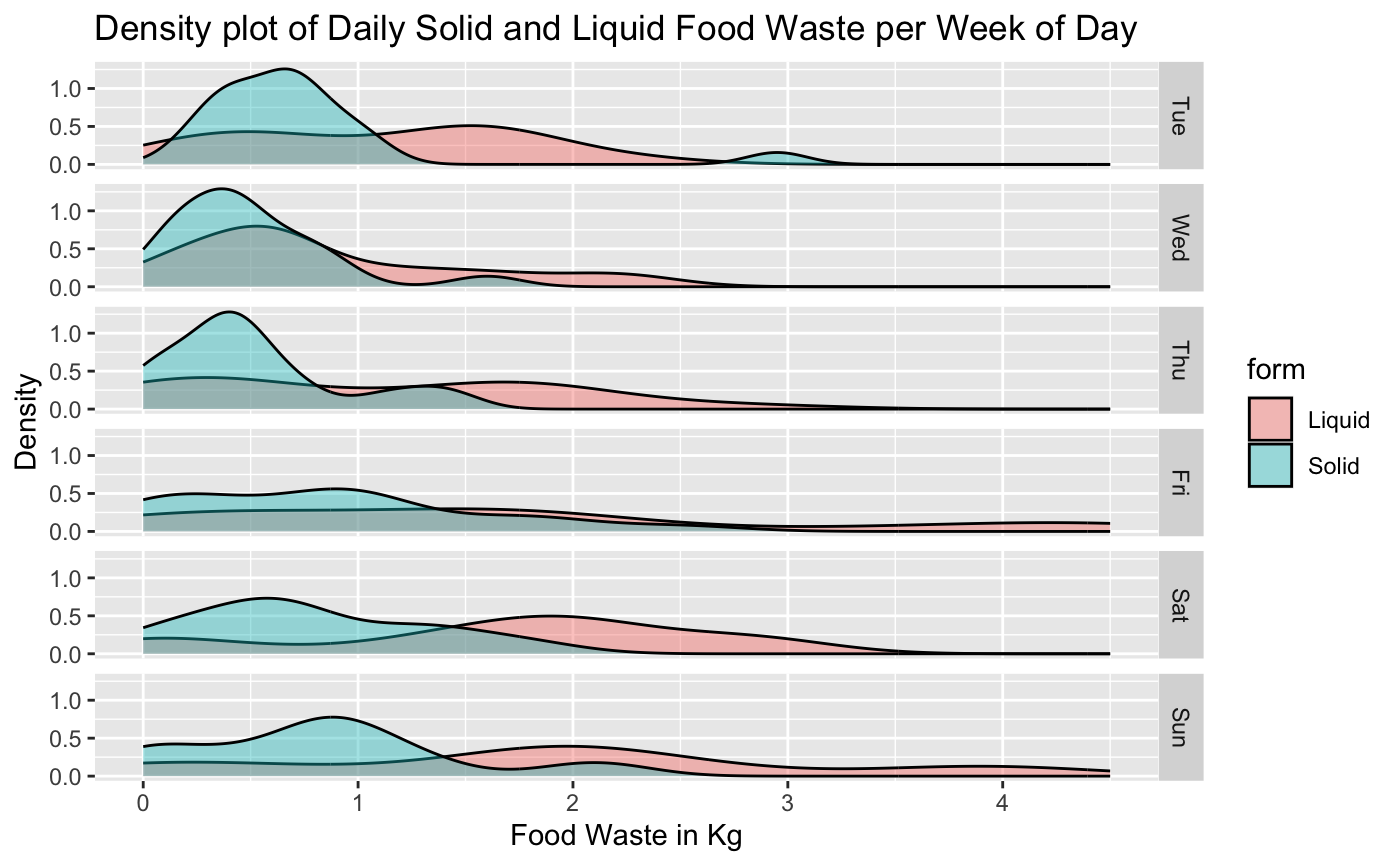
\includegraphics[width=0.4\textwidth,height=\textheight]{weekFW.png} &
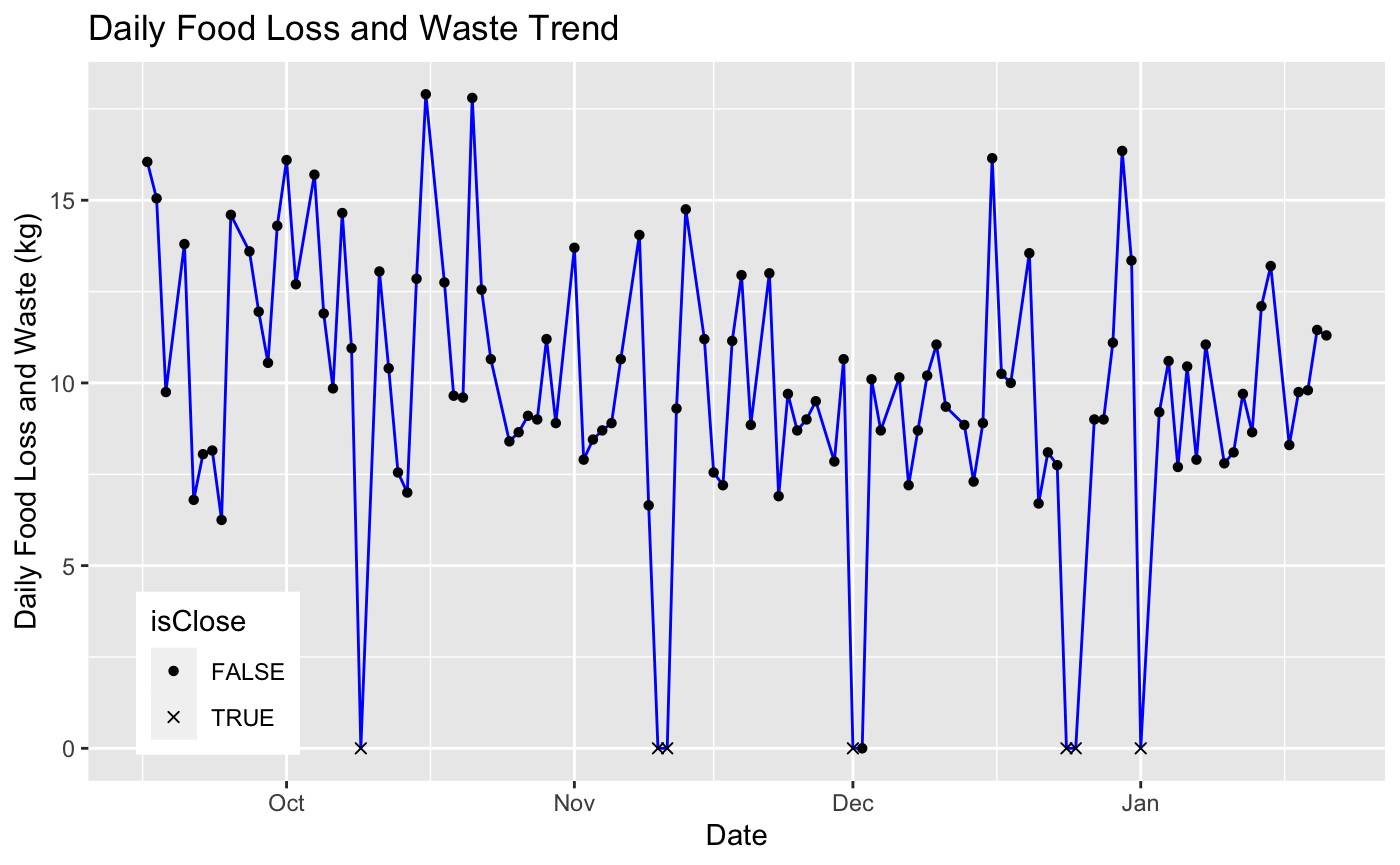
\includegraphics[width=0.4\textwidth,height=\textheight]{tsFLW.png} \\
\bottomrule()
\end{longtable}
\end{block}
\end{frame}

\begin{frame}{Expected Results}
\protect\hypertarget{expected-results-4}{}
\begin{block}{TODO}
\protect\hypertarget{todo}{}
\begin{itemize}
\tightlist
\item
  Develop potential causes of FLW (Weather and Calendar Effects)
\item
  Calculate the average rate of food loss and waste
\item
  Estimate econbomic and environmental effects
\end{itemize}
\end{block}
\end{frame}

\hypertarget{acknowledgements}{%
\section{Acknowledgements}\label{acknowledgements}}

\begin{frame}{Acknowledgements}
\protect\hypertarget{acknowledgements-1}{}
I would like to express my gratitude to my supervisor, Dr.~Balbinder
Deo, and to the committee member for his support and encouragement in my
initial thesis development. I would also like to thank the University of
Northern British Columbia and Prince George for allowing me an
opportunity to pursue graduate studies.
\end{frame}

\hypertarget{references}{%
\section{References}\label{references}}

\begin{frame}{References}
\protect\hypertarget{references-1}{}
{[}1{]} Gustavsson, J. (Ed.). (2011). Global food losses and food waste:
extent, causes and prevention; study conducted for the International
Congress Save Food! at Interpack 2011, {[}16 - 17 May{]}, Düsseldorf,
Germany. Food and Agriculture Organization of the United Nations.\\
{[}2{]} Blakeney, M. (2019). Food loss and food waste: Causes and
solutions.\\
{[}3{]} National Zero Waste Council. (2016). A tax incentive to prevent
food waste in Canada. NZWC. Retrieved October 12, 2021, from
\url{http://www.nzwc.ca/Documents/NZWC-} TaxIncentiveBackgrounder.pdf.\\
{[}4{]} Gooch, M., Bucknell, D., LaPlain, D., Dent, B., Whitehead, P.,
Felfel, A., Nikkel, L., \& Maguire, M. (2019). The avoidable crisis of
food waste: Technical report. Value Chain Management International and
Second Harvest, Ontario, Canada, 122.\\
\end{frame}

\begin{frame}{References}
\protect\hypertarget{references-2}{}
{[}5{]} Retrieved on August 20, 2022 from:
\url{https://www2.gov.bc.ca/gov/content/environment/waste-management/food-and-organic-waste/prevent-}
food-waste\\
{[}6{]} Aschemann-Witzel, J., de Hooge, I., Amani, P., Bech-Larsen, T.,
\& Oostindjer, M. (2015). Consumer-related food waste: Causes and
potential for action. Sustainability (Switzerland), 7(6), 6457--6477.\\
{[}7{]} Lusk, J. L., \& Ellison, B. (2017). A note on modelling
household food waste behaviour. Applied Economics Letters, 24(16),
1199--1202.\\
{[}8{]} Nahman, A., de Lange, W., Oelofse, S., \& Godfrey, L. (2012).
The costs of household food waste in South Africa. Waste Management,
32(11), 2147--2153.\\
\end{frame}

\begin{frame}{References}
\protect\hypertarget{references-3}{}
{[}9{]} Von Massow, M., Parizeau, K., Gallant, M., Wickson, M., Haines,
J., Ma, D. W. L., Wallace, A., Carroll, N., \& Duncan, A. M. (2019).
Valuing the multiple impacts of household food waste. Frontiers in
Nutrition, 6, 143.\\
{[}10{]} Ishangulyyev, R., Kim, S., \& Lee, S. H. (2019). Understanding
food loss and waste---why are we losing and wasting food?. Foods, 8(8),
297.\\
{[}11{]} Harrell, F. E., Lee, K. L., Califf, R. M., Pryor, D. B., \&
Rosati, R. A. (1984). Regression modelling strategies for improved
prognostic prediction. Statistics in Medicine, 3(2), 143--152.
\url{https://doi.org/10.1002/sim.4780030207}\\
{[}12{]} Green, S. B. (1991). How many subjects does it take to do a
regression analysis. Multivariate behavioral research, 26(3), 499-510.\\
\end{frame}

\end{document}
